\documentclass[8pt]{beamer}
%\documentclass{beamer}
\usepackage[nobglogo]{beamerthemedmi-owled}
\usepackage{graphicx}
\usepackage{dl}
\usepackage{mls}
\usepackage{xspace}
\usepackage{amssymb}
\usepackage{amsfonts}
\usepackage{amsthm}
\usepackage{amsmath}
\usepackage{enumerate}
\usepackage{color}
\usepackage{url}
\usepackage{xspace}

\mode<presentation>
{
  \usetheme{dmi-owled}
  %\usetheme{Warsaw}
  % or ...

  \setbeamercovered{transparent}
  % or whatever (possibly just delete it)
}


\usepackage[english]{babel}
% or whatever

\usepackage[latin1]{inputenc}
% or whatever

\newcommand{\TBox}{{\tt TBox}}
\newcommand{\ABox}{{\tt ABox}}
\newcommand{\Ont}{\mathcal{O}}

\newcommand{\highl}[1]{\textcolor{red}{\underline{#1}}}


%TERMS

%Concepts
\newcommand{\Mortal}{\mathtt{Mortal}}
\newcommand{\Human}{\mathtt{Human}}
\newcommand{\Male}{\mathtt{Male}}
\newcommand{\Female}{\mathtt{Female}}
\newcommand{\Man}{\mathtt{Man}}
\newcommand{\Woman}{\mathtt{Woman}}

%Roles
\newcommand{\relative}{\mathtt{relativeOf}}
\newcommand{\child}{\mathtt{childOf}}
\newcommand{\grandchild}{\mathtt{grandChildOf}}
\newcommand{\age}{\mathtt{age}}
\newcommand{\owner}{\mathtt{ownerOf}}

\newcommand{\Person}{\mathtt{Person}}
\newcommand{\partner}{\mathtt{partnerOf}}
\newcommand{\parent}{\mathtt{parentOf}} 
\newcommand{\ancestor}{\mathtt{ancestorOf}} 
\newcommand{\descendant}{\mathtt{descendantOf}}

%OTHER TERMS
\newcommand{\father}{\mathtt{father}} 
\newcommand{\grandfather}{\mathtt{grandfather}} 

%INDIVIDUALS
\newcommand{\Alice}{Alice}
\newcommand{\Bob}{Bob}
\newcommand{\Charlie}{Charlie}
\newcommand{\Dana}{Dana}
\newcommand{\Edwige}{Edwige}
\newcommand{\Fido}{Fido}

%KNOWLEDGE BASES
\newcommand{\KBsets}{\mathcal{K}_{\mathcal{L}}}
\newcommand{\KBlcons}{\widehat{\mathcal{K}}_{\mathcal{L}}}
\newcommand{\KBsetsq}{\mathcal{K}^{q}_\mathcal{L}}
\newcommand{\KBdl}{\mathcal{K}}
\newcommand{\KBzerozero}{\mathcal{K}_{\mathcal{S},0}}
\newcommand{\KBzeroone}{\mathcal{K}_{\mathcal{S},1}}
\newcommand{\KBzero}{\mathcal{K}_{\mathcal{S}}}
\newcommand{\KBtra}{\mathcal{K}'_{\mathcal{S}}}
\newcommand{\KBirr}{\mathcal{K}''_{\mathcal{S}}}
\newcommand{\KBq}{\mathcal{K}^{q}_{\mathcal{S}}}
\newcommand{\KBel}{\mathcal{K_E}}
\newcommand{\Kcand}{\mathcal{O}}

%ADDITIONALS
% Queries
\newcommand{\TestCases}{\mathit{T}}
\newcommand{\italian}{\mathtt{Italian}}
\newcommand{\withitrel}{\mathtt{WithItRelative}}
\newcommand{\withitanc}{\mathtt{ItDescendant}}

% Tests
%\newcommand{\testpassed}{\textsf{Y}}
\newcommand{\testpassed}{\textsf{Y}}
\newcommand{\testfailed}{\bf{\textsf{N}}}

\title{Adding \emph{Semantics} to Ontologies}

\author{Cristiano Longo}
\institute{Dipartimento di Matematica e Informatica, Universit\`a di Catania, Italy \\
\url{mailto://longo@dmi.unict.it}
}

\date{SOD2014}

\begin{document}
\maketitle
\setcounter{tocdepth}{1}
%\tableofcontents

\section{Introduction}

\begin{frame}
\frametitle{About}

This talk is about the word \emph{Semantic} in the ``Semantic Web.''
\vspace{\baselineskip}

It will provides some basic theoretical notions for a better
understanding of Semantic Web technologies (in particular OWL).
\end{frame}

\begin{frame}
\frametitle{Topics}

Some answers for the following questions will be provided:
\begin{itemize}[<+->]
 \item How can we represent knowledge? (ontologies)
 \item Which tools the Semantic Web framework offer to this end? (OWL)
 \item How representing knowledge with these tools can be useful? (reasoning)
\end{itemize}
\end{frame}

\begin{frame}
\frametitle{Notice}
  For the sake of readability and for historical reason, we will use
  notation and terminology from \emph{Descriptio Logics}, which
  underpin Semantic Web languages (in particular OWL). 
\end{frame}

\section{Knowledge Representation}

\begin{frame}
 \Large{Representing Knowledge in Logic and Computer Science}
\end{frame}


\begin{frame}
\frametitle{Ontologies}
  An \emph{ontology} is a (partial) description of the world.
  \vspace{\baselineskip}
  
  Usually, it is a finite set of statements such as, for example,
  \begin{itemize}
   \item human beings are mortals,
   \item Alice is the Bob's mother,
   \item Federico II was an emperor.
  \end{itemize}
\end{frame}


\begin{frame}
\frametitle{Basics}
  A knowledge domain is described in terms of
  \begin{itemize}
   \item \emph{individuals}, to indicate domain items ($\Alice$, $\Bob$, \ldots),
    \item \emph{concepts} (aka \emph{classes}), which denote sets of domain objects ($\Person$, $\Male$,  \ldots), and
    \item \emph{roles} (aka \emph{properties}), which are relations on domain items ($\parent$, $\partner$, \ldots).  
  \end{itemize}
\end{frame}

\begin{frame}
\frametitle{Vocabulary and Assertions}
  Each ontology is divided into two parts:

  \begin{itemize}
    \item the \TBox (vocabulary), in which \emph{vocabulary terms} for concepts (i.e. sets) 
    and roles (i.e. relations) are defined, and
    \item the \ABox, which contains statements (namely, \emph{assertions}) about real world items.
  \end{itemize}
    \vspace{\baselineskip}
    
  \uncover<2->{
  \begin{center}
    \begin{tabular}{|l|l|}
    \hline
    \TBox & \emph{Concepts:} $\Male$, $\Female$,$\Human$,$\Woman$, $\Man$. \\ 
    & \emph{Roles:} $\relative$, $\child$, $\grandchild$. \\      
    \hline
    \ABox & $\Woman(\Alice)$, $\Man(\Bob)$, $\Alice\,\relative\,\Bob$, \\
     & $\Alice\,\child\,\Charlie$. \\
    \hline
  \end{tabular}
    \end{center}
  }
\end{frame}

\begin{frame}
\frametitle{Open World Assumption}

Facts not explicitly mentioned in the ontology are \emph{not} assumed to be false,
their truth value is just unknown.
\vspace{\baselineskip}

\uncover<2->{
In general, no one has complete knowledge.  
}

\begin{center}
  \begin{tabular}{|l|l|}
    \hline
    \TBox & \emph{Concepts:} $\Male$, $\Female$,$\Human$,$\Woman$, $\Man$. \\ 
    & \emph{Roles:} $\relative$, $\child$, $\grandchild$. \\      
    \hline
    \ABox & $\Woman(\Alice)$, $\Man(\Bob)$, $\Alice\,\relative\,\Bob$, \\
     & $\Alice\,\child\,\Charlie$. \\
    \hline
  \end{tabular}
\end{center}

\begin{itemize}
 \item What is the kinship relation between $\Alice$ and $\Bob$? $\Charlie\,\child\,\Alice$?
 \item Is $\Charlie$ a man? Is $\Charlie$ a human being?
 \uncover<2->{
 \item What about other persons in the world?
 }
\end{itemize}
\end{frame}

\begin{frame}
\frametitle{Open World Assumption - Interpretations}
All the \emph{possible worlds} must be taken into account.

\uncover<2->{
An \emph{interpretation} associates sets, relations, and items of a
given \emph{domain} (i.e. Universe) $\Delta$ to concepts and roles 
in the vocabulary.
}

\uncover<3->{
For example:
\[
 \begin{array}{rcl|l}
 \Delta & := & \{ \Alice, \Bob, \Charlie, \Dana, \Edwige\} & \Alice\,\child\,\Bob\\
 \Human & := & \{ \Alice, \Bob, \Charlie, \Dana \} & \Charlie\,\relative\,\Bob\\
 \Female & := & \{ \Alice, \Dana, \Edwige \} \\
 \Male & := & \{\Bob, \Charlie \}\\
 \Woman & := & \{ \Alice, \Dana \} \\
 \Man & := & \{\Bob \Charlie \} \\
 \end{array}
\]
}

\end{frame}

\begin{frame}
\frametitle{Open World Assumption - Models (1/2)}
Roughly speaking, an interpretation is a \emph{model} for an ontology
if it does not contradicts the ontology itself
\vspace{\baselineskip}

For example:
\[
 \begin{array}{rcl|l}
 \Delta & := & \{ \Alice, \Bob, \Charlie, \Dana, \Edwige\} & \Alice\,\child\,\Charlie\\
 \Human & := & \{ \Alice, \Bob, \Charlie, \Dana \} & \Charlie\,\relative\,\Bob\\
 \Female & := & \{ \Alice, \Dana, \Edwige \} \\
 \Male & := & \{\Bob, \Charlie \}\\
 \Woman & := & \{ \Alice, \Dana \} \\
 \Man & := & \{\Bob \Charlie \} \\
 \end{array}
\]

is a model for

\begin{center}
  \begin{tabular}{|l|l|}
    \hline
    \TBox & \emph{Concepts:} $\Male$, $\Female$,$\Human$,$\Woman$, $\Man$. \\ 
    & \emph{Roles:} $\relative$, $\child$, $\grandchild$. \\      
    \hline
    \ABox & $\Woman(\Alice)$, $\Man(\Bob)$, $\Alice\,\relative\,\Bob$, \\
     & $\Alice\,\child\,\Charlie$. \\
    \hline
  \end{tabular}
\end{center}
\end{frame}

\begin{frame}
\frametitle{Open World Assumption - Models (2/2)}
Wherease the following is not.
\vspace{\baselineskip}

\[
 \begin{array}{rcl|l}
 \Delta & := & \{ \Alice, \Bob, \Charlie, \Dana, \Edwige\} & \Alice\,\relative\,\Charlie\\
 \Human & := & \{ \Alice, \Bob, \Charlie, \Dana \} & \Charlie\,\relative\,\Bob\\
 \Female & := & \{ \Alice, \Dana, \Edwige \} \\
 \Male & := & \{\Bob, \Charlie \}\\
 \Woman & := & \{ \Alice, \Dana \} \\
 \Man & := & \{\Bob \Charlie \} \\
 \end{array}
\]

\phantom{is a model for}

\begin{center}
  \begin{tabular}{|l|l|}
    \hline
    \TBox & \emph{Concepts:} $\Male$, $\Female$,$\Human$,$\Woman$, $\Man$. \\ 
    & \emph{Roles:} $\relative$, $\child$, $\grandchild$. \\      
    \hline
    \ABox & $\Woman(\Alice)$, $\Man(\Bob)$, $\Alice\,\relative\,\Bob$, \\
     & 	\alert{$\Alice\,\child\,\Charlie$}. \\
    \hline
  \end{tabular}
\end{center}
\end{frame}


%TODO ontologies can be merged and reused

\begin{frame}
\frametitle{Constraints}

How to to associate \emph{meanings} to vocabulary 
terms:
\vspace{\baselineskip}

by means of \emph{constraints} (placed in the \TBox) expressed in a mathematical
fashion involving concepts, roles, individuals. 

\begin{example}
\[
\begin{array}{ll}
\Human \Issub \Mortal & \mbox{all persons are mortal;} \\
\\
\Woman \equiv \Human \sqcap \Female & \mbox{women are female human beings;} \\
\\
\child \circ \child \subseteq \grandchild & \mbox{the child of the child is the grandchild.} 
\end{array}
\] 
\end{example}
\vspace{\baselineskip}

\uncover<2->{
In general, the syntax of a \emph{Knowledge Representation Language} is 
characterized by the types of constraints it allows, mainly in term of
\emph{operators} (eg. $\sqcap$, $\circ$, \ldots).
}
\end{frame}

\section{Semantic Web}

\begin{frame}
 \Large{Representing Knowledge the Semantic Web}
\end{frame}

\begin{frame}
 \frametitle{Semantic Web Stack}
 Semantic Web technologies are \emph{stratified}.
 \vspace{\baselineskip}
 
 \phantom{Some of such technologies are knowledge representation languages.}
 \vspace{\baselineskip}
 
 \begin{figure}
 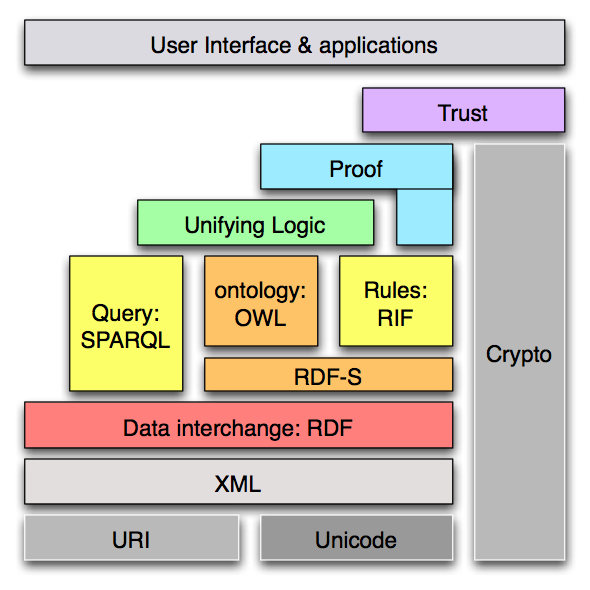
\includegraphics[height=150px]{SemWebStack-tbl-2006a.png}
 \caption{The Semantic Web stack}
 \end{figure}

\end{frame}

\begin{frame}
 \frametitle{Representing Knowledge the Semantic Web}
 Semantic Web technologies are \emph{stratified}.
 \vspace{\baselineskip}
 
 Some of these are knowledge representation languages.
 \vspace{\baselineskip}
 
 \begin{figure}
 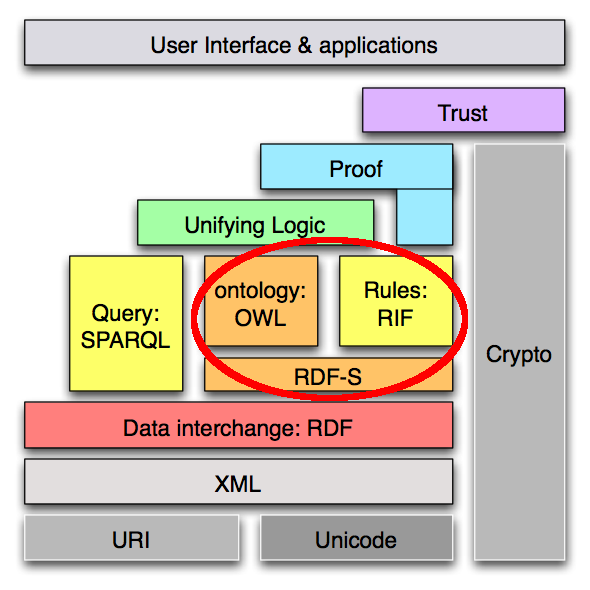
\includegraphics[height=150px]{SemWebStack-tbl-2006a_kr.png}
 \caption{The Semantic Web stack}
 \end{figure}

\end{frame}

\begin{frame}
 \frametitle{OWL}
 \emph{OWL} is the concise name of the \emph{Web Ontology Language}, currently at version 2.
 \vspace{\baselineskip}
 \begin{center}
  \url{http://www.w3.org/TR/2012/REC-owl2-primer-20121211/}
 \end{center}

 
 Three different \emph{profiles} (fragments) have been defined for it (see \url{http://www.w3.org/TR/2012/REC-owl2-profiles-20121211/}):
 \begin{itemize}
  \item \emph{OWL-RL} quite good expressive power;
  \item \emph{OWL-QL} for large $\ABox$;
  \item \emph{OWL-EL} very efficient, also in presence of large $\TBox$.
 \end{itemize}
 \vspace{\baselineskip}
 
 
 \uncover<2->{
  Here we consider OWL-EL. 
 }
\end{frame}

\begin{frame}
 \frametitle{OWL-EL and \elplusplus} 
 OWL-EL is underpinned by the description logic \elplusplus.
 It has been devided in the biohealth domain (SNOMED-CT).
 \vspace{\baselineskip}
 
 \uncover<2->{
 \emph{Concept constructors} of $\elplusplus$ are:
 \begin{itemize}
  \item $\top$ \emph{(every)thing};
  \item $\bot$ \emph{nothing};
  \item $\{a\}$ \emph{nominal}, the set with only member $a$;
  \item $\exists R.C$ \emph{existential restriction}, all those 
  items related with some element in $C$;
  \item $C \sqcap D$ \emph{conjunction}, all the members of
  both $C$ and $D$;
  \item \emph{concrete domains} (e.g. $\age > 18$).
 \end{itemize}
 }
 
  \uncover<3->{
    Such constructors can be used to form complex concepts, e.g.
\[
 \exists \child.\{\Fido\} := \{ \Edwige \}, \quad \exists \child. (\Male \sqcap \Human).
\]    
  }

\end{frame}

\begin{frame}
 \frametitle{\elplusplus concepts - Thing}
 Let us consider the following \emph{possible world} (interpretation)
 \[
 \begin{array}{rcl|l}
  \Delta & := & \{ \Alice, \Bob, \Charlie, \Dana, \Edwige, \Fido \} & \Alice\,\child\,\Charlie \\
  \Human & := & \{ \Alice, \Bob, \Charlie, \Dana \} & \Alice\,\child\,\Dana\\
  \Female & := & \{ \Alice, \Dana, \Edwige \} & \Edwige\,\child\,\Fido\\
  \Male & := & \{ \Bob, \Charlie, \Fido \} & \Charlie\,\relative\,\Bob \\
  & & & \Bob\,\owner\,\Fido .
 \end{array}
\]

\[
 \phantom{\top := \{ \Alice, \Bob, \Charlie, \Dana, \Edwige, \Fido \}}
\]

 \begin{center}
  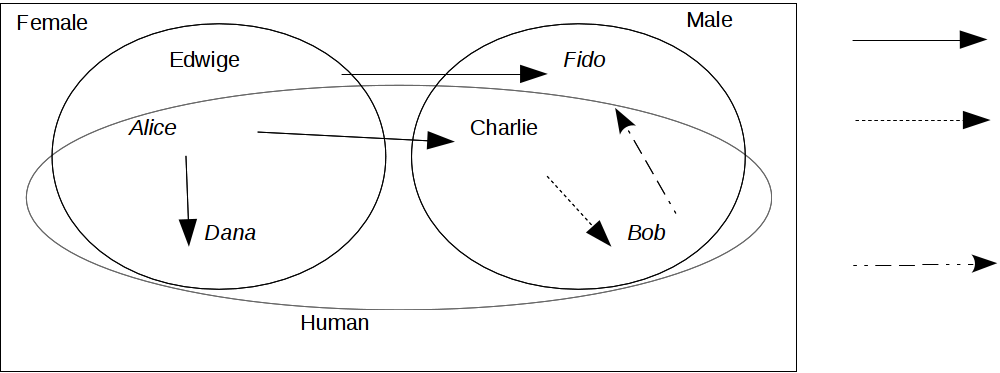
\includegraphics[width=300px, keepaspectratio]{images/exbase_big.png}  
 \end{center}
\end{frame}

\begin{frame}
 \frametitle{\elplusplus concepts - Thing}
 Let us consider the following \emph{possible world}
 \[
 \begin{array}{rcl|l}
  \Delta & := & \{ \Alice, \Bob, \Charlie, \Dana, \Edwige, \Fido \} & \Alice\,\child\,\Charlie \\
  \Human & := & \{ \Alice, \Bob, \Charlie, \Dana \} & \Alice\,\child\,\Dana\\
  \Female & := & \{ \Alice, \Dana, \Edwige \} & \Edwige\,\child\,\Fido\\
  \Male & := & \{ \Bob, \Charlie, \Fido \} & \Charlie\,\relative\,\Bob \\
  & & & \Bob\,\owner\,\Fido .
 \end{array}
\]

\[
 \top := \{ \Alice, \Bob, \Charlie, \Dana, \Edwige, \Fido \}
\]

 \begin{center}
  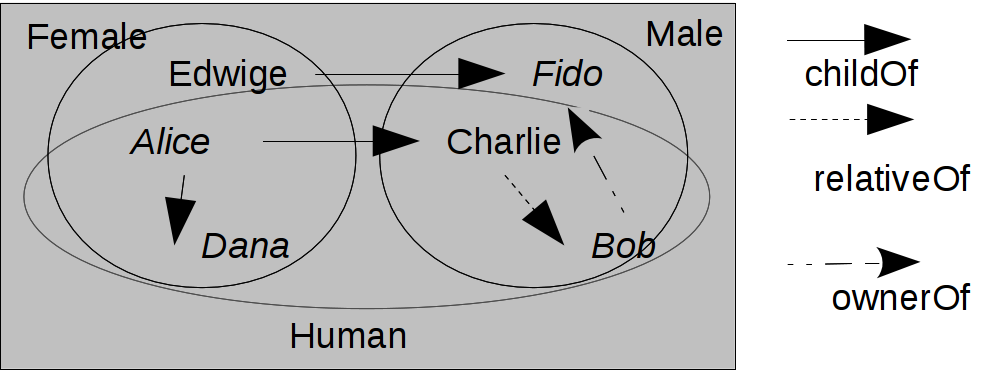
\includegraphics[width=300px, keepaspectratio]{images/extop_big.png}  
 \end{center}
\end{frame}

\begin{frame}
 \frametitle{\elplusplus concepts - Nothing}
 Let us consider the following \emph{possible world}
 \[
 \begin{array}{rcl|l}
  \Delta & := & \{ \Alice, \Bob, \Charlie, \Dana, \Edwige, \Fido \} & \Alice\,\child\,\Charlie \\
  \Human & := & \{ \Alice, \Bob, \Charlie, \Dana \} & \Alice\,\child\,\Dana\\
  \Female & := & \{ \Alice, \Dana, \Edwige \} & \Edwige\,\child\,\Fido\\
  \Male & := & \{ \Bob, \Charlie, \Fido \} & \Charlie\,\relative\,\Bob \\
  & & & \Bob\,\owner\,\Fido .
 \end{array}
\]

\[
 \bot := \emptyset
\]

 \begin{center}
  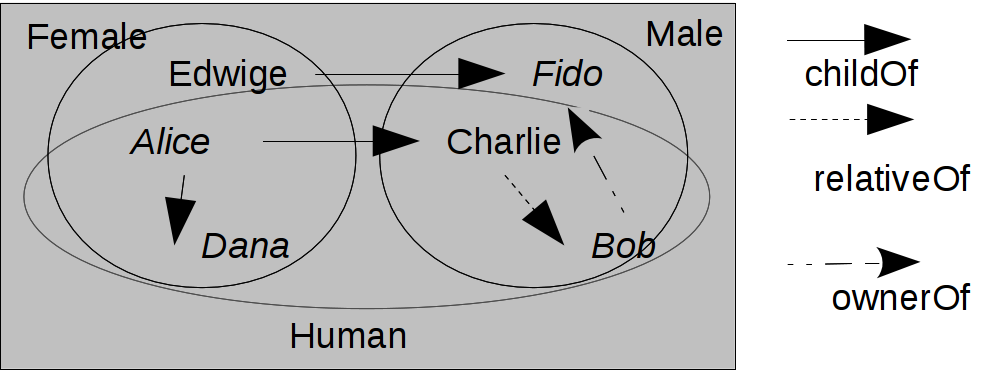
\includegraphics[width=300px, keepaspectratio]{images/extop_big.png}  
 \end{center}
\end{frame}

\begin{frame}
 \frametitle{\elplusplus concepts - Nominal}
 Let us consider the following \emph{possible world}
 \[
 \begin{array}{rcl|l}
  \Delta & := & \{ \Alice, \Bob, \Charlie, \Dana, \Edwige, \Fido \} & \Alice\,\child\,\Charlie \\
  \Human & := & \{ \Alice, \Bob, \Charlie, \Dana \} & \Alice\,\child\,\Dana\\
  \Female & := & \{ \Alice, \Dana, \Edwige \} & \Edwige\,\child\,\Fido\\
  \Male & := & \{ \Bob, \Charlie, \Fido \} & \Charlie\,\relative\,\Bob \\
  & & & \Bob\,\owner\,\Fido .
 \end{array}
\]

\[
 \{ \Alice \} := \{ \Alice \}
\]

 \begin{center}
  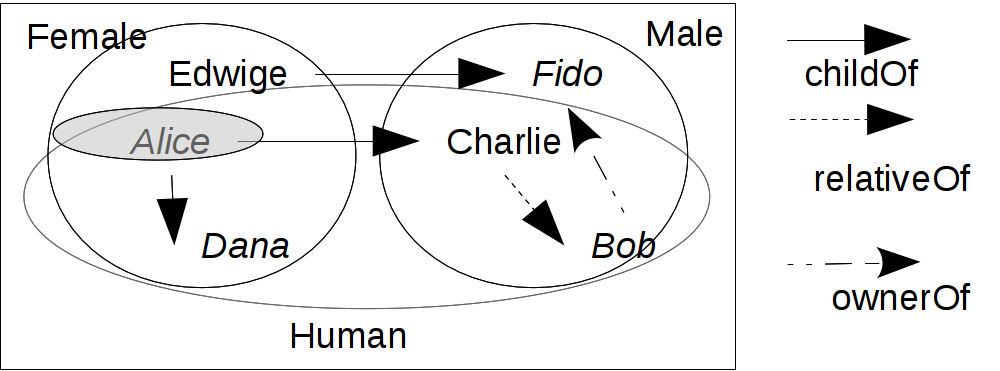
\includegraphics[width=300px, keepaspectratio]{images/exsing_big.png}  
 \end{center}
\end{frame}

\begin{frame}
 \frametitle{\elplusplus concepts - existential restriction}
 Let us consider the following \emph{possible world}
 \[
 \begin{array}{rcl|l}
  \Delta & := & \{ \Alice, \Bob, \Charlie, \Dana, \Edwige, \Fido \} & \Alice\,\child\,\Charlie \\
  \Human & := & \{ \Alice, \Bob, \Charlie, \Dana \} & \Alice\,\child\,\Dana\\
  \Female & := & \{ \Alice, \Dana, \Edwige \} & \Edwige\,\child\,\Fido\\
  \Male & := & \{ \Bob, \Charlie, \Fido \} & \Charlie\,\relative\,\Bob \\
  & & & \Bob\,\owner\,\Fido .
 \end{array}
\]

\[
 \exists \owner.\Male := \{ \Bob \}
\]

 \begin{center}
  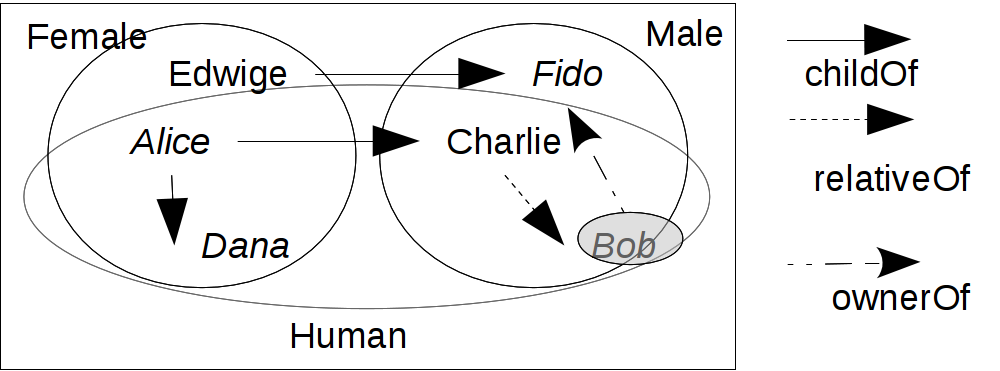
\includegraphics[width=300px, keepaspectratio]{images/exexists_big.png}  
 \end{center}
\end{frame}

\begin{frame}
 \frametitle{\elplusplus concepts - conjunction (intersection)}
 Let us consider the following \emph{possible world}
 \[
 \begin{array}{rcl|l}
  \Delta & := & \{ \Alice, \Bob, \Charlie, \Dana, \Edwige, \Fido \} & \Alice\,\child\,\Charlie \\
  \Human & := & \{ \Alice, \Bob, \Charlie, \Dana \} & \Alice\,\child\,\Dana\\
  \Female & := & \{ \Alice, \Dana, \Edwige \} & \Edwige\,\child\,\Fido\\
  \Male & := & \{ \Bob, \Charlie, \Fido \} & \Charlie\,\relative\,\Bob \\
  & & & \Bob\,\owner\,\Fido .
 \end{array}
\]

\[
 \Female \sqcap \Human := \{ \Alice, \Dana \}
\]

 \begin{center}
  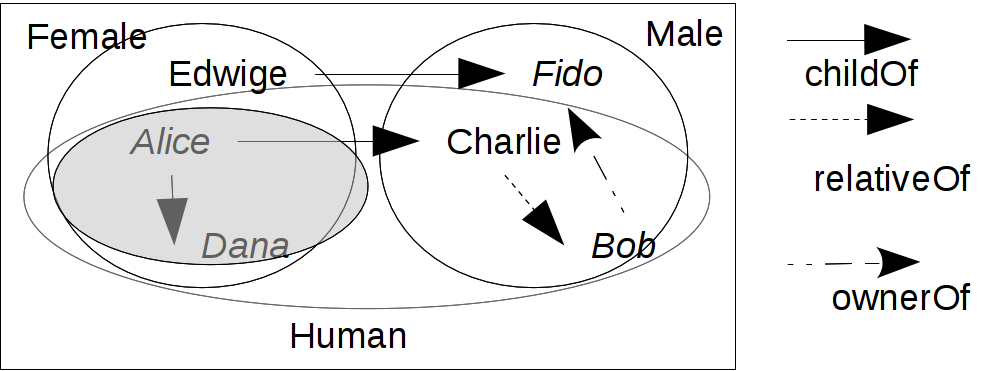
\includegraphics[width=300px, keepaspectratio]{images/exint_big.png}  
 \end{center}
\end{frame}


\begin{frame}
 \frametitle{\elplusplus concepts - complex concepts}
 Let us consider the following \emph{possible world}
 \[
 \begin{array}{rcl|l}
  \Delta & := & \{ \Alice, \Bob, \Charlie, \Dana, \Edwige, \Fido \} & \Alice\,\child\,\Charlie \\
  \Human & := & \{ \Alice, \Bob, \Charlie, \Dana \} & \Alice\,\child\,\Dana\\
  \Female & := & \{ \Alice, \Dana, \Edwige \} & \Edwige\,\child\,\Fido\\
  \Male & := & \{ \Bob, \Charlie, \Fido \} & \Charlie\,\relative\,\Bob \\
  & & & \Bob\,\owner\,\Fido .
 \end{array}
\]

\[
 \exists \child.\{\Fido\} := \{ \Edwige \}
\]

 \begin{center}
  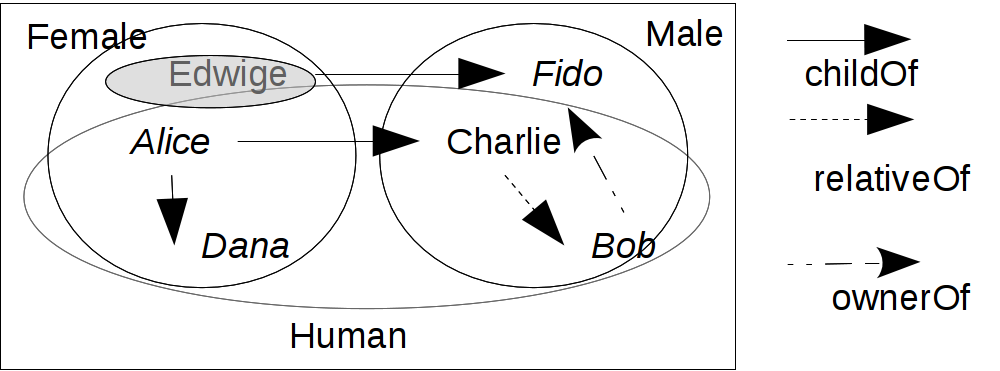
\includegraphics[width=300px, keepaspectratio]{images/excomplex_big.png}  
 \end{center}
\end{frame}

\begin{frame}
 \frametitle{\elplusplus constraints}
 Constraints allowed in $\elplusplus$ $\TBox$ are of the types:
 \begin{itemize}
  \item $C \Issub D$ every member of $C$ is a member of $D$ as well;
  \item $C \equiv D$ the sets $C$ and $D$ coincide;
  \item $R_1 \circ \ldots \circ R_n \Issub S$ the \emph{composition} of $R_1$, \ldots, $R_n$ is a subrelation of
  $S$;
  \item $\dom(R) \Issub C$ if $x$ is related to $y$ by $R$, then $x$ must be a member of $C$;
  \item $\range(R) \Issub C$ if $x$ is related to $y$ by $R$, then $y$ must be a member of $C$.  
 \end{itemize}
\end{frame}

\begin{frame}
 \frametitle{\elplusplus constraints - subsumption}
 The following is a \emph{model} for
 \[
    \Man \Issub \Human
 \]
 
 \[
 \begin{array}{rcl|l}
  \Delta & := & \{ \Alice, \Bob, \Charlie, \Dana, \Edwige, \Fido \} & \Alice\,\child\,\Charlie \\
  \Human & := & \{ \Alice, \Bob, \Charlie, \Dana \} & \Alice\,\child\,\Dana\\
  \Female & := & \{ \Alice, \Dana, \Edwige \} & \Edwige\,\child\,\Fido\\
  \Male & := & \{ \Bob, \Charlie, \Fido \} & \Charlie\,\relative\,\Bob \\
  \Man & := & \{ \Bob, \Charlie \} & \Bob\,\owner\,\Fido . \\
 \end{array}
\]

 \begin{center}
  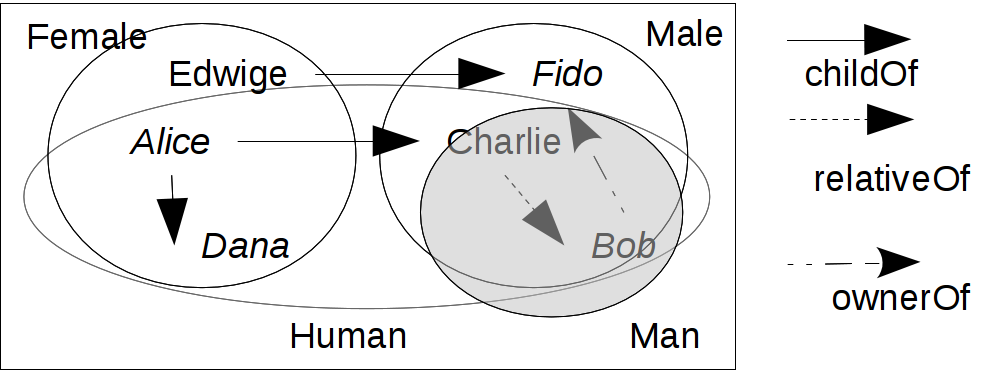
\includegraphics[width=300px, keepaspectratio]{images/exsub_big.png}  
 \end{center}
\end{frame}

\begin{frame}
 \frametitle{\elplusplus constraints - equivalence}
 The same is a model for
 \[
    \Man \equiv \Human \sqcap \Male
 \]
 
 \[
 \begin{array}{rcl|l}
  \Delta & := & \{ \Alice, \Bob, \Charlie, \Dana, \Edwige, \Fido \} & \Alice\,\child\,\Charlie \\
  \Human & := & \{ \Alice, \Bob, \Charlie, \Dana \} & \Alice\,\child\,\Dana\\
  \Female & := & \{ \Alice, \Dana, \Edwige \} & \Edwige\,\child\,\Fido\\
  \Male & := & \{ \Bob, \Charlie, \Fido \} & \Charlie\,\relative\,\Bob \\
  \Man & := & \{ \Bob, \Charlie \} & \Bob\,\owner\,\Fido . \\
 \end{array}
\]

 \begin{center}
  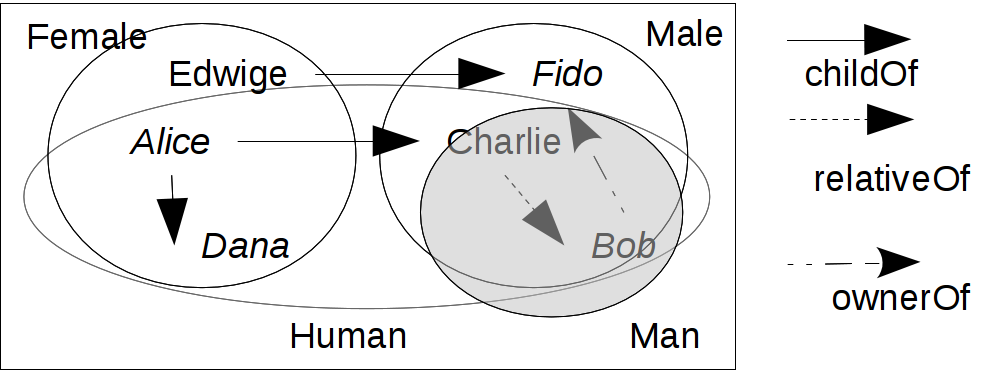
\includegraphics[width=300px, keepaspectratio]{images/exsub_big.png}  
 \end{center}
\end{frame}

\begin{frame}
 \frametitle{\elplusplus constraints - composition (1/2)}
 Let us consider
 \[
 \begin{array}{cr}
    \child \circ \relative \subseteq \relative & \mbox{the child of a relative is a relative as well.}
 \end{array}
 \]

 The following is \emph{not} a model for this constraint ($\Alice$ should be relative of $\Charlie$):
 \[
 \begin{array}{rcl|l}
  \Delta & := & \{ \Alice, \Bob, \Charlie, \Dana, \Edwige, \Fido \} & \Alice\,\child\,\Charlie \\
  \Human & := & \{ \Alice, \Bob, \Charlie, \Dana \} & \Alice\,\child\,\Dana\\
  \Female & := & \{ \Alice, \Dana, \Edwige \} & \Edwige\,\child\,\Fido\\
  \Male & := & \{ \Bob, \Charlie, \Fido \} & \Charlie\,\relative\,\Bob \\
  \Man & := & \{ \Bob, \Charlie \} & \Bob\,\owner\,\Fido . \\
 \end{array}
\]

 \begin{center}
  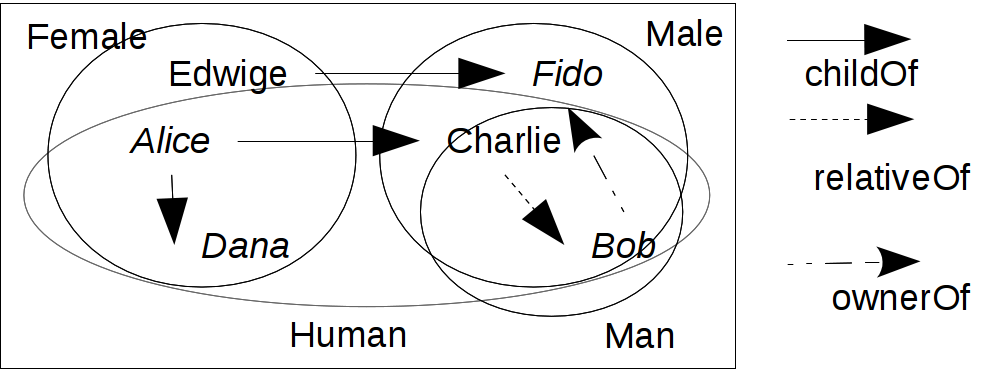
\includegraphics[width=300px, keepaspectratio]{images/exbaseman_big.png}  
 \end{center}
\end{frame}

\begin{frame}
 \frametitle{\elplusplus constraints - composition (2/2)}
 A model for $\child \circ \relative \subseteq \relative$ is:

 The following is \emph{not} a model for this constraint ($\Alice$ should be relative of $\Bob$):
 \[
 \begin{array}{rcl|l}
  \Delta & := & \{ \Alice, \Bob, \Charlie, \Dana, \Edwige, \Fido \} & \Alice\,\child\,\Charlie \\
  \Human & := & \{ \Alice, \Bob, \Charlie, \Dana \} & \Alice\,\child\,\Dana\\
  \Female & := & \{ \Alice, \Dana, \Edwige \} & \Edwige\,\child\,\Fido\\
  \Male & := & \{ \Bob, \Charlie, \Fido \} & \Charlie\,\relative\,\Bob \\
  \Man & := & \{ \Bob, \Charlie \} & \Bob\,\owner\,\Fido \\
  & & & \Alice\,\relative\,\Bob . \\
 \end{array}
\]

 \begin{center}
  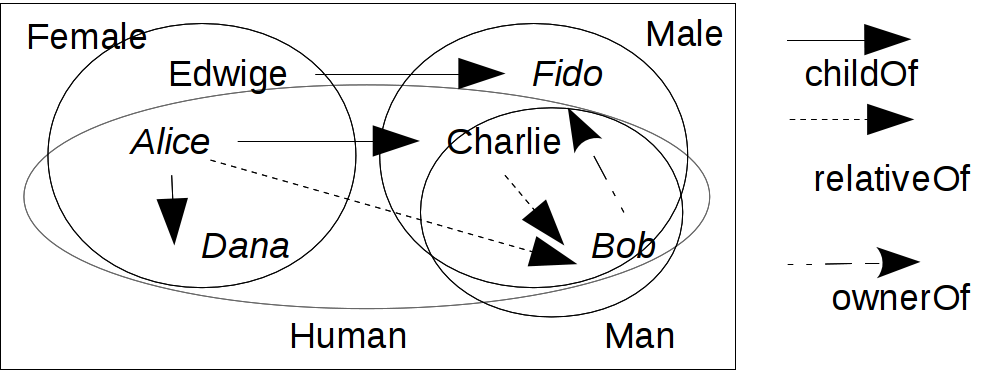
\includegraphics[width=300px, keepaspectratio]{images/excomp_big.png}  
 \end{center}
\end{frame}

\begin{frame}
 \frametitle{\elplusplus constraints - domain}
 It is a model for 
 \[
 \begin{array}{cr}
    \dom(\owner) \Issub \Human & \mbox{all owners are humans.}
 \end{array}
 \]
 
 \[
 \begin{array}{rcl|l}
  \Delta & := & \{ \Alice, \Bob, \Charlie, \Dana, \Edwige, \Fido \} & \Alice\,\child\,\Charlie \\
  \Human & := & \{ \Alice, \Bob, \Charlie, \Dana \} & \Alice\,\child\,\Dana\\
  \Female & := & \{ \Alice, \Dana, \Edwige \} & \Edwige\,\child\,\Fido\\
  \Male & := & \{ \Bob, \Charlie, \Fido \} & \Charlie\,\relative\,\Bob \\
  \Man & := & \{ \Bob, \Charlie \} & \Bob\,\owner\,\Fido . \\
 \end{array}
\]

 \begin{center}
  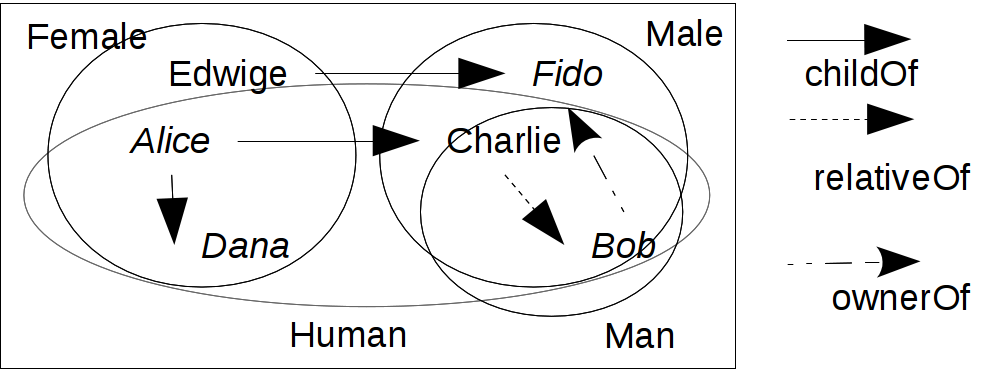
\includegraphics[width=300px, keepaspectratio]{images/exbaseman_big.png}  
 \end{center}
\end{frame}

\begin{frame}
 \frametitle{\elplusplus constraints - range}
 But this is \emph{not} a model for 
 \[
 \begin{array}{cr}
    \range(\owner) \Issub \Human & \mbox{all \emph{owned} are humans.}
 \end{array}
 \]

 \[
 \begin{array}{rcl|l}
  \Delta & := & \{ \Alice, \Bob, \Charlie, \Dana, \Edwige, \Fido \} & \Alice\,\child\,\Charlie \\
  \Human & := & \{ \Alice, \Bob, \Charlie, \Dana \} & \Alice\,\child\,\Dana\\
  \Female & := & \{ \Alice, \Dana, \Edwige \} & \Edwige\,\child\,\Fido\\
  \Male & := & \{ \Bob, \Charlie, \Fido \} & \Charlie\,\relative\,\Bob \\
  \Man & := & \{ \Bob, \Charlie \} & \Bob\,\owner\,\Fido . \\
 \end{array}
\]

 \begin{center}
  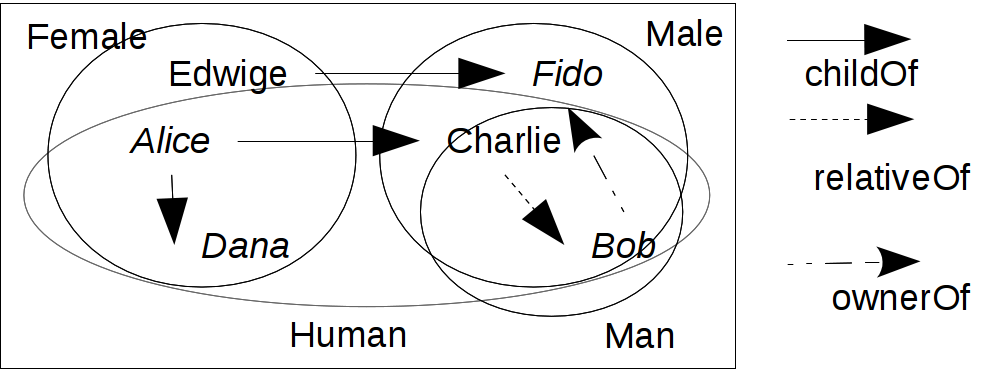
\includegraphics[width=300px, keepaspectratio]{images/exbaseman_big.png}  
 \end{center}
\end{frame}

\section{Reasoning}

\begin{frame}
\Large{Using Knowledge encoded in \elplusplus} 
\end{frame}


\begin{frame}
 \frametitle{Reasoning}
 Defining a formal semantics enables some \emph{reasoning} task to be
 performed automatically.

 Here we will see
 \begin{itemize}
  \item \emph{consistency checking}, to check the absence of logical errors,
  \item \emph{inferencing}, to extract hidden knowledge.
 \end{itemize}
\end{frame}


\begin{frame}
 \frametitle{Reasoning - Consistency}
 
 An ontology is \emph{consistent} if a possible world which \emph{matches} it exists.
 \vspace{\baselineskip}
 
 Let us consider the following ontology:
 \[
  \begin{array}{|l|l|}
   \hline
   \TBox & \ABox\\
   \hline
   \Woman \equiv \Female \sqcap \Human & \Woman(\Alice)\\
   \Man \equiv \Male \sqcap \Human & \Man(\Charlie)\\
   \child\,\circ\,\relative \subseteq \relative &  \Alice\,\child\,\Charlie\\
   \dom(\owner) \Issub \Human & \Charlie\,\relative\,\Bob\\
   & \Bob\,\owner\,\Fido\\
   \hline
  \end{array}
 \]
 
 It is consistent (see before for a model).
 
\begin{center}
  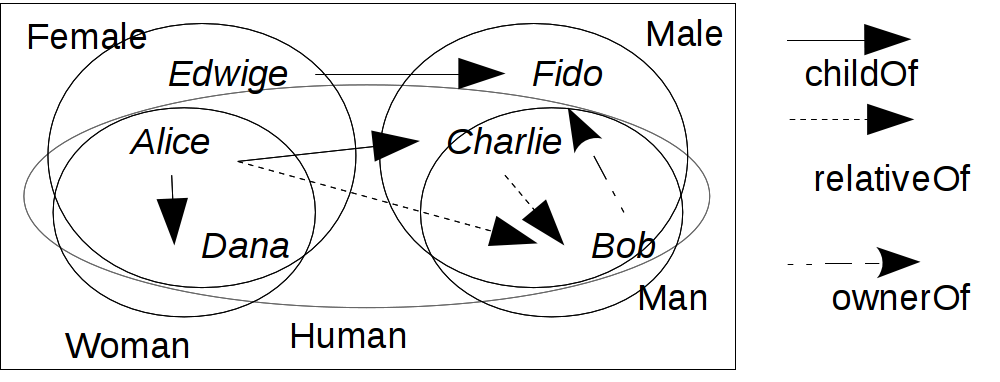
\includegraphics[width=300px, keepaspectratio]{images/exbasemanwoman_big.png}  
\end{center}

\end{frame}

\begin{frame}
 \frametitle{Reasoning - Consistency - example 2}
 
 The following one is \emph{not} consistent.
 \[
  \begin{array}{|l|l|}
   \hline
   \TBox & \ABox\\
   \hline
   \Woman \equiv \Female \sqcap \Human & \Woman(\Alice)\\
   \Man \equiv \Male \sqcap \Human & \Man(\Charlie)\\
   \child\,\circ\,\relative \subseteq \relative &  \Alice\,\child\,\Charlie\\
   \dom(\owner) \Issub \Human & \Charlie\,\relative\,\Bob\\
   \alert{\Male \sqcap \Female \equiv \bot}& \Bob\,\owner\,\Fido\\
   & \alert{\Female(\Bob)}\\
   \hline
  \end{array}
 \]
 $\Bob$ must be $\Male$, as it is a $\Man$, all men are $\Male$ and $\Male$ and $\Female$ are
 disjoint.
\end{frame}

\begin{frame}
 \frametitle{Reasoning - Consistency - example 3}
 
 The following one is \emph{not} consistent.
 \[
  \begin{array}{|l|l|}
   \hline
   \TBox & \ABox\\
   \hline
   \Woman \equiv \Female \sqcap \Human & \Woman(\Alice)\\
   \Man \equiv \Male \sqcap \Human & \Man(\Charlie)\\
   \child\,\circ\,\relative \subseteq \relative &  \Alice\,\child\,\Charlie\\
   \alert{\dom(\owner) \Issub \Human} & \Charlie\,\relative\,\Bob\\
   \alert{\Human \sqcap \Edwige \equiv \bot}& \Bob\,\owner\,\Fido\\
   & \alert{\Edwige\,\owner\,\Fido}\\
   \hline
  \end{array}
 \]
 $\Edwige$ can't be the owner of $\Fido$ because $\Edwige$ is not a member of $\Human$.
\end{frame}

\begin{frame}
 \frametitle{Reasoning - Inference}

 \emph{Inferences} retrieves all the assertions which hold in \emph{all} the possible models.
 
 \[
  \begin{array}{|l|l|}
   \hline
   \TBox & \ABox\\
   \hline
   \Woman \equiv \Female \sqcap \Human & \Woman(\Alice)\\
   \Man \equiv \Male \sqcap \Human & \Man(\Charlie)\\
   \child\,\circ\,\relative \subseteq \relative &  \Alice\,\child\,\Charlie\\
   \dom(\owner) \Issub \Human & \Charlie\,\relative\,\Bob\\
   & \Bob\,\owner\,\Fido\\
   \hline
   Inferred\,Statements & \\
   \phantom{\Female(\Alice)} & \\
   \phantom{\Human(\Alice)} & \\
   \phantom{\Male(\Charlie)} & \\
   \phantom{\Human(\Charlie)} & \\
   \phantom{\Alice\,\relative\,\Bob} & \\
   \phantom{\Human(\Bob)} & \\
   \hline
  \end{array}
 \]
\end{frame}

\begin{frame}
 \frametitle{Reasoning - Inference}

 \emph{Inferences} retrieves all the assertions which hold in \emph{all} the possible models.
 
 \[
  \begin{array}{|l|l|}
   \hline
   \TBox & \ABox\\
   \hline
   \alert{\Woman \equiv \Female \sqcap \Human} & \alert{\Woman(\Alice)}\\
   \Man \equiv \Male \sqcap \Human & \Man(\Charlie)\\
   \child\,\circ\,\relative \subseteq \relative &  \Alice\,\child\,\Charlie\\
   \dom(\owner) \Issub \Human & \Charlie\,\relative\,\Bob\\
   & \Bob\,\owner\,\Fido\\
   \hline
   Inferred\,Statements & \\
   \alert{\Female(\Alice)}& \\
   \alert{\Human(\Alice)}& \\
   \phantom{\Male(\Charlie)} & \\
   \phantom{\Human(\Charlie)} & \\
   \phantom{\Alice\,\relative\,\Bob} & \\
   \phantom{\Human(\Bob)} & \\
   \hline
  \end{array}
 \]
\end{frame}

\begin{frame}
 \frametitle{Reasoning - Inference}

 \emph{Inferences} retrieves all the assertions which hold in \emph{all} the possible models.
 
 \[
  \begin{array}{|l|l|}
   \hline
   \TBox & \ABox\\
   \hline
   \Woman \equiv \Female \sqcap \Human & \Woman(\Alice)\\
   \alert{\Man \equiv \Male \sqcap \Human} & \alert{\Man(\Charlie)}\\
   \child\,\circ\,\relative \subseteq \relative &  \Alice\,\child\,\Charlie\\
   \dom(\owner) \Issub \Human & \Charlie\,\relative\,\Bob\\
   & \Bob\,\owner\,\Fido\\
   \hline
   Inferred\,Statements & \\
   \Female(\Alice)& \\
   \Human(\Alice)& \\
   \alert{\Male(\Charlie)} & \\
   \alert{\Human(\Charlie)} & \\
   \phantom{\Alice\,\relative\,\Bob} & \\
   \phantom{\Human(\Bob)} & \\
   \hline
  \end{array}
 \]
\end{frame}

\begin{frame}
 \frametitle{Reasoning - Inference}

 \emph{Inferences} retrieves all the assertions which hold in \emph{all} the possible models.
 
 \[
  \begin{array}{|l|l|}
   \hline
   \TBox & \ABox\\
   \hline
   \Woman \equiv \Female \sqcap \Human & \Woman(\Alice)\\
   \Man \equiv \Male \sqcap \Human & \Man(\Charlie)\\
   \alert{\child\,\circ\,\relative \subseteq \relative} &  \alert{\Alice\,\child\,\Charlie}\\
   \dom(\owner) \Issub \Human & \alert{\Charlie\,\relative\,\Bob}\\
   & \Bob\,\owner\,\Fido\\
   \hline
   Inferred\,Statements & \\
   \Female(\Alice)& \\
   \Human(\Alice)& \\
   \Male(\Charlie) & \\
   \Human(\Charlie) & \\
   \alert{\Alice\,\relative\,\Bob} & \\
   \phantom{\Human(\Bob)} & \\
   \hline
  \end{array}
 \]
\end{frame}

\begin{frame}
 \frametitle{Reasoning - Inference}

 \emph{Inferences} retrieves all the assertions which hold in \emph{all} the possible models.
 
 \[
  \begin{array}{|l|l|}
   \hline
   \TBox & \ABox\\
   \hline
   \Woman \equiv \Female \sqcap \Human & \Woman(\Alice)\\
   \Man \equiv \Male \sqcap \Human & \Man(\Charlie)\\
   \child\,\circ\,\relative \subseteq \relative &  \Alice\,\child\,\Charlie\\
   \alert{\dom(\owner) \Issub \Human} & \Charlie\,\relative\,\Bob\\
   & \alert{\Bob\,\owner\,\Fido}\\
   \hline
   Inferred\,Statements & \\
   \Female(\Alice)& \\
   \Human(\Alice)& \\
   \Male(\Charlie) & \\
   \Human(\Charlie) & \\
   \Alice\,\relative\,\Bob & \\
   \alert{\Human(\Bob)} & \\
   \hline
  \end{array}
 \]
\end{frame}

\begin{frame}
\begin{center}
 \Large{Thank You!}
 \vspace{\baselineskip}
 
 (questions?)
\end{center}

\end{frame}


%TODO fino qua
\end{document}